\section{Numerical solution techniques}\label{sec:numerical_techniques}
The discussion to this point has outlined the formulation of the \methodAcronym\ method. We now consider numerical solution techniques. 
\EP{I think passive voice is fine in this instance, it reads easier}
As \methodAcronym\ displays commonalities with optimal
control problems, a large existing body of work can be leveraged. This section
discuses a variety of such techniques and outlines how they can be used to
solve the \methodAcronym\ system. We focus primarily on 
%\KTC{earlier we kept
%saying 
%direct (i.e.,
%	discretize-then-optimize) and indirect (i.e., optimize-then-discretize).
%	Let's be consistent when we re-introduce it here.}
direct (discretize-the-optimize) and indirect (optimize-then-discretize) for \spatialAcronym\ trial subspaces, 
and then briefly outline direct and indirect methods for \spaceTimeAcronym\ trial subspaces. 

\subsection{\spatialAcronym: direct and indirect methods}
Numerical techniques to
solve optimal control problems can be classified as either
\textit{direct} or \textit{indirect}
methods~\cite{conway_optimalcontrolreview}.  Direct methods eschew the first order optimality conditions
~\eqref{eq:lspg_continuous}--\eqref{eq:lspg_bcs} and, instead, ``directly" solve the optimization problem~\eqref{eq:tclsrm} by first
numerically discretizing the system and objective functional and ``transcribing"
the infinite dimensional problem into a finite-dimensional nonlinear
programming (optimization) problem. Direct approaches thus ``discretize then optimize."
Indirect methods, on the other hand, leverage the calculus of variations to
derive the Euler--Lagrange equations, which comprise the first-order
optimality conditions~\eqref{eq:lspg_continuous}--\eqref{eq:lspg_bcs} associated with the objective 
functional. Indirect methods then solve (numerically) the Euler--Lagrange equations. Thus, indirect methods ``optimize then discretize," and 
solve the optimization problem
``indirectly". A variety of discretization/solution techniques are possible for both direct and indirect methods. Collocation methods,
finite elements, spectral methods, shooting methods, etc., are all examples of
plausible solution techniques.  

In the present context, we investigate both direct and indirect methods to solve \methodAcronym\ with \spatialAcronym\ trial
subspaces. We consider: 
\begin{itemize} \item \textit{Direct Methods (discretize-then-optimize)}: Discretize and then optimize approaches are outlined for linear multistep methods. 
\item \textit{Indirect methods (optimize-then-discretize)}: An indirect method leveraging the forward-backward sweep algorithm is outlined 
to solve~\eqref{eq:lspg_continuous}-\eqref{eq:lspg_bcs}. 
\end{itemize} 
We emphasize that a variety of other approaches exist. Future work will comprise a detailed exploration
of additional approaches.
Section~\ref{sec:direct}  outlines direct solution approaches based on linear
multistep methods, while Section~\ref{sec:indirect} outlines the indirect
solution approach. 



\subsection{\spatialAcronym\ trial subspaces: direct solution approach}\label{sec:direct} 

Direct approaches solve optimization problem~\eqref{eq:tclsrm} by
``transcribing" the infinite dimensional optimization problem into a finite
dimensional one by discretizing the state and objective functional in time.
The minimization problem is then reformulated as a (non)linear programming, or
optimization, problem. A variety of direct solution approaches exist, 
including collocation approaches, spectral  methods, and genetic algorithms.  

In the context of \spatialAcronym\ trial subspaces, the most straightforward direct solution approach consists of the 
following steps: (1) numerically discretize the FOM ODE (and hence the
\textit{integrand} of the objective function in problem~\eqref{eq:obj_gen_slab}) and 
(2) select a numerical quadrature rule to evaluate the \textit{integral} in~\eqref{eq:obj_gen_slab}.
To this end, we define a time grids
$\{\timeWindowArg{n}{i}\}_{i=0}^{\nstepsArg{n}}\subseteq[\timeStartArg{n},\timeEndArg{n}]$,
$n=1,\ldots,\nslabs$ that
satisfy 
$\timeStartArg{n}=\timeWindowArg{n}{0} \le \cdots \le \timeWindowArg{n}{\nstepsArg{n}} 
 = \timeEndArg{n}$.
%\KTC{use cdots, not
%hdots or ldots. Don't use $\defeq$ for the first and last times; these are
%just equalities, i.e., you happen to set them equal to those values, but they
%aren't identically the same:}
Figure~\ref{fig:slab_fig2} depicts such a discretization.
We now outline the direct solution approach for linear-multistep schemes; we note that the formulation for
other time-integration methods (e.g., Runge--Kutta) follows closely. 
\begin{figure} 
\begin{centering} 
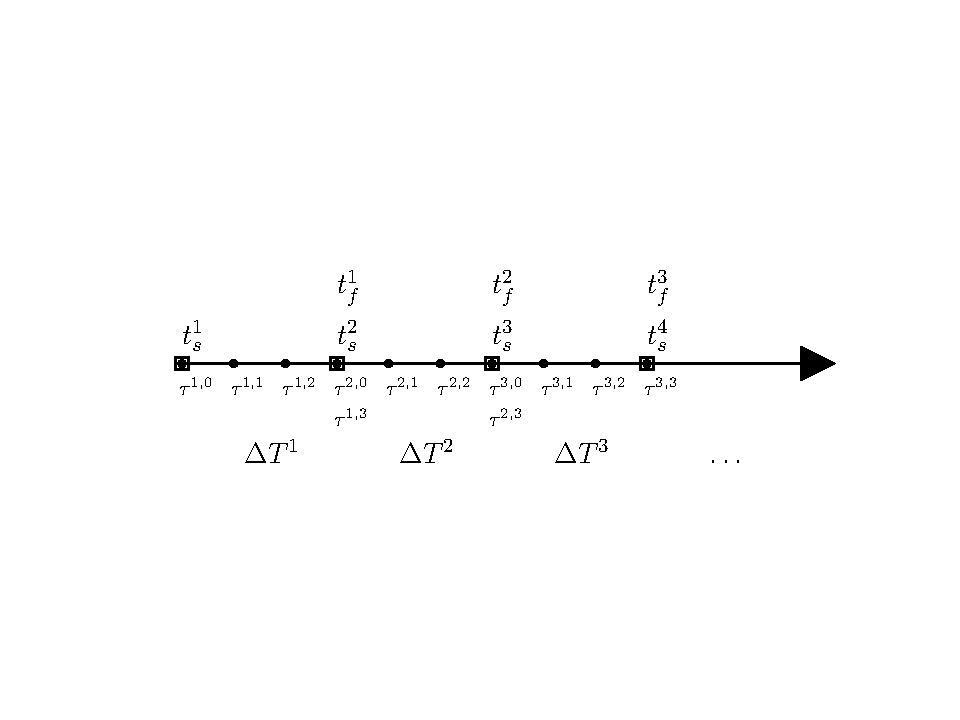
\includegraphics[trim={0.0cm 4.5cm 0cm 3cm},clip,width=1.0\textwidth]{figs/time_grid_timesteps.pdf} 
	\caption{Depiction of the $\nstepsArg{n}+1$ time instances over each window. In the figure, $\nstepsArg{n} = 2$ for all $n$.} 
\label{fig:slab_fig2} 
\end{centering} 
\end{figure}
%We now outline several commonly employed temporal discretization 
%schemes, specifically linear multistep and collocation (Runge--Kutta) methods, that leverage this time-grid to discretize the FOM ODE and 
%objective functional.  

%\subsubsection{Temporal Discretization of the FOM ODE}
%To develop the direct solution approach, we first outline several 
%commonly employed methods used to discretize the FOM ODE, and then 
%subsequently demonstrate how these techniques can be used to discretize 
%and solve Eq.~\ref{eq:obj_gen_slab}. To develop the direct solution approach, 
%we start by dividing each time slab $[\timeStartArg{n},\timeEndArg{n}]$ into
%$\nstepsArg{n}$ strictly increasing time-step instances described by,
%$\{\timeWindowArg{n}{i}\}_{i=0}^{\nstepsArg{n}}$, with  \begin{align*}
%&\timeWindowArg{n}{0} \le \ldots \le \timeWindowArg{n}{\nstepsArg{n}} , \\
%&\timeWindowArg{n}{0} \defeq \timeStartArg{n}, \\
%&\timeWindowArg{n}{\nstepsArg{n}} \defeq \timeEndArg{n}. 
%%\timeWindowArg{n}{0} = \timeStartArg{n}, \timeWindowArg{n}{\nstepsArg{n}} =
%%\timeEndArg{n}
%\end{align*}
\subsubsection{Linear multistep schemes}
Linear multistep schemes approximate the solution at time instance $\timeWindowArg{n}{i}$ using the previous $k$ time instances.  
%Discretizing the FOM ODE~\eqref{eq:FOM} with a linear $k$-step scheme at the $i$th time-instance over the $n$th time slab yields,
%\begin{equation}\label{eq:kstep}
%\sum_{j=0}^{\lmsWidthArg{n}{i}} \alpha_j \stateFOMDiscreteArg{n,i-j} = \Delta t^{n,i} \sum_{j=0}^{\lmsWidthArg{n}{i}} \beta_j \velocity(\stateFOMDiscreteArg{n,i-j}),
%\end{equation}
Employing a linear multistep method to discretize the FOM ODE yields the FOM O$\Delta$E over the $n$th window,
\KTC{Note: the notation here is not consistent with what was defined earlier
for a discrete residual. See email.}
\begin{align*}
&\residLMSArg{n,i} (\stateFOMDiscreteArg{n,i};\stateFOMDiscreteArg{n,i-1},\ldots,\stateFOMDiscreteArg{n,i-\lmsWidthArg{n}{i}}) = \bz, \qquad i=1,\ldots,\nstepsArg{n}, \\
&\stateFOMDiscreteArg{n,0} = \begin{cases}
\stateFOMDiscreteArg{n-1,\nstepsArg{n-1}} & n = 2,\ldots,\nslabs, \\
\stateFOMIC & n=1, \end{cases}
\end{align*}
where $\stateFOMDiscreteArg{n,i} (\approx
\stateFOMArg{}{\timeWindowArg{n}{i}})
\in \RR{\fomdim}$ and $\residLMSArg{n,i}$ denotes the FOM O$\Delta$E
residual over the $i$th time instance of the $n$th window  
defined as
\begin{align*}
\residArg{n,i} &: (\stateyDiscreteArgnt{i};\stateyDiscreteArgnt{i-1},\ldots,\stateyDiscreteArgnt{i-\lmsWidthArg{n}{i}}) \mapsto  \frac{1}{\Delta t^{n,i}} \sum_{j=0}^{\lmsWidthArg{n}{i}} \alpha^{n,i}_j \stateyDiscreteArgnt{i-j} -  \sum_{j=0}^{\lmsWidthArg{n}{i}} \beta^{n,i}_j \velocity(\stateyDiscreteArgnt{i-j},\timeWindowArg{n}{i-j}) \\
               &: \RR{\fomdim} \otimes \RR{\lmsWidthArg{n}{i}+1} \rightarrow \RR{\fomdim}. 
\end{align*} 
Here, $\Delta t^{n,i} \defeq \timeWindowArg{n}{i} - \timeWindowArg{n}{i-1}$
denotes the time step, $\lmsWidthArg{n}{i}$ denotes the number of time steps employed by the scheme at the $i$th time instance over the $n$th window and
$\alpha^{n,i}_j,\beta^{n,i}_j\in\RR{}$ denote coefficients that 
define the specific type of multistep scheme. To handle the case where the linear multistep method employs time instances from the previous window(s), we enforce the condition on the indices $(n,i) = (n-1,\nstepsArg{n-1}+i)$ for $i<0$. 
%\begin{remark}\label{remark:LMS}
%For notational simplicity, we assume the linear multistep method employs time
%	instances from only within the current time window. In general, the linear
%	multistep method at the $n$th window could be designed to employ multiple
%	time instances from previous time windows. \KTC{What are the implications of
%	this? I suggest removing this and adding a simple condition, maybe with a
%	footnote.}
%\end{remark}
%Employing a linear multistep method for temporal discretization of the FOM ODE leads to the FOM O$\Delta$E over the $n$th slab,
%\begin{align*}
%&\residLMSArg{n,i} (\stateFOMDiscreteArg{n,i},\ldots,\stateFOMDiscreteArg{n,i-k^n(i)}) = \bz, \qquad i=1,\ldots,\nstepsArg{n}, \\
%&\stateArgnt{n,0} = \begin{cases}
%\stateFOMDiscreteArg{n-1,\nstepsArg{n-1}} & n = 2,\ldots,\nslabs, \\
%\stateFOMIC & n=1, \end{cases}
%\end{align*}
%where $\residLMSArg{n,i}$ is the discrete linear multistep residual over the $i$th time-step instance of the $n$th slab,
%\begin{align*}
%\residArg{n,i} &: (\stateyDiscreteArgnt{n,i},\ldots,\stateyDiscreteArgnt{n,i-k(i)}) \mapsto  \frac{1}{\Delta t^{n,i}} \sum_{j=0}^{\lmsWidthArg{n}{i}} \alpha_j \stateyDiscreteArgnt{n,i-j} -  \sum_{j=0}^{\lmsWidthArg{n}{i}} \beta_j \velocity(\stateyDiscreteArgnt{n,i-j}),
%\\
%               &: \RR{\fomdim} \otimes \RR{k(i)} \rightarrow \RR{\fomdim}. 
%\end{align*} 
\EP{In the process of reworking this slightly, need to take care for the case where we are employing multiple time steps 
from the previous window. Still cleaning up}
\methodAcronym\ with the direct approach and a linear multistep method sequentially computes the solutions
$\approxstateDiscreteArg{n,1},\ldots,\approxstateDiscreteArg{n,\nstepsArg{n}}$,
$n=1,\ldots,\nslabs$ that satisfy
%	\KTC{What is $\genstate^{n-1}(\timeEndArg{n-1} ) $ doing here? Two problems
%	(1) there is no notion of a generalized coordinate $\genstate$ yet, and (2)
%	this should be the discrete solution, not the exact solution evaluated at
%	the final time.} \EP{You are correct, I think there is an error now in the minimize term though. It was $\in \trialspace\otimes \RR{\lmsWidthArg{n}{i}+1}$, it should be $\trialspace\otimes \RR{\nstepsArg{n}+1}$}
\begin{align*}
	&\underset{(\stateyDiscreteArgnt{1},\ldots,\stateyDiscreteArgnt{\nstepsArg{n}}) \in \trialspace\otimes \RR{\nstepsArg{n}{i}}}{\text{minimize } }
\objectiveArgLMS{n} (\stateyDiscreteArgnt{1},\ldots,\stateyDiscreteArgnt{\nstepsArg{n}}). 
%%& \text{subject to} \hspace{0.2 in}  \stateyDiscreteArg{0} =
%%\begin{cases} \basisspaceArg{n} \spatialICDiscrete + \stateInterceptArg{n}& n = 2,\ldots,\nslabs,\\
%\basisspaceArg{1} \genstateICOne  + \stateInterceptArg{1}& n=1. \end{cases} 
\end{align*}
%Employing a linear multistep method allows the objective \textit{functional}~\eqref{eq:obj} to be replaced with the objective \textit{function}
%\EP{Had to change the definition of the objective function to reflect stepping back into previous window}
In the above, $\objectiveArgLMS{n}$ is the discrete objective function at the $n$th time window and is defined as
\begin{equation}\label{eq:obj_lms}
\begin{split} 
\objectiveArgLMS{n} &\vcentcolon (\stateyDiscreteArgnt{1},\ldots,\stateyDiscreteArgnt{\nstepsArg{n}}) \mapsto
\frac{1}{2} \sum_{i=1}^{\nstepsArg{n}} \quadWeightsLMSScalarArg{n}{i} [\residArg{n,i}(\stateyDiscreteArgnt{i};\ldots, \stateyDiscreteArgnt{i-\lmsWidthArg{n}{i})})]^T  \stweightingMatArgt{n}{\timeWindowArg{n}{i}} \residArg{n,i}(\stateyDiscreteArgnt{i};\ldots, \stateyDiscreteArgnt{i-\lmsWidthArg{n}{i}}), \\
&\vcentcolon \RR{\fomdim} \otimes \RR{\nstepsArg{n}} \rightarrow
\RR{}_+, 
\end{split}
\end{equation}
where $\quadWeightsLMSScalarArg{n}{i} \in \RRplus$ are quadrature weights and, for $i \le 0$ in $\objectiveArgLMS{n}$, we take
\begin{equation}\label{eq:wls_spatial_direct_args}
\stateyDiscreteArgnt{i}  \equiv 
\begin{cases}
\basisspaceArg{n} \basisspaceTArg{n} (\approxstateDiscreteArg{n-1,\nstepsArg{n-1}+i} - \stateInterceptArg{n}) + \stateInterceptArg{n} & n = 2,\ldots,\nslabs,  \\
\basisspaceArg{n} \basisspaceTArg{n} (\stateFOMIC - \stateInterceptArg{n}) + \stateInterceptArg{n} & n = 1.
\end{cases}
\end{equation}
Note that the boundary conditions are automatically satisfied by Eq.~\eqref{eq:wls_spatial_direct_args}.

%where 
%\begin{align*}
%\residArg{n,i} &: (\stateyArgnt{n,i},\ldots,\stateyArgnt{n,i-k(i)}) \mapsto  \sum_{j=0}^k \alpha_j \stateyArgnt{n,i-j} = \Delta t^{n,i} \sum_{j=0}^k \beta_j \velocity(\stateyArgnt{n,i-j}),
%\\
%               &: \RR{\fomdim} \otimes \RR{k(i)} \rightarrow \RR{\fomdim}, 
%\end{align*} 
%is the discrete residual resulting from the linear multistep scheme and 
%\methodAcronym\ solves the minimization problem over each time window, 
%\begin{align*}
%&\approxstateDiscreteArg{n,0},\ldots,\approxstateDiscreteArg{n,\nstepsArg{n}} = \underset{\stateyDiscreteArgnt{n,0},\ldots,\stateyDiscreteArgnt{n,\nstepsArg{n}} \in \trialspace}{\text{arg\,min } }
%\objectiveArgLMS{n} (\stateyDiscreteArgnt{n,0},\ldots,\stateyDiscreteArgnt{n,\nstepsArg{n}}) \\
%& \text{subject to} \hspace{0.2 in}  \approxstateDiscreteArg{n,0} =
%\begin{cases} \approxstateDiscreteArg{n-1,\nstepsArg{n-1}} & n = 2,\ldots,\nslabs,\\
%\approxstateIC & n=1. \end{cases} \end{align*}
	Equivalently, \methodAcronym\ sequentially computes the generalized
	coordinates
	$\genstateDiscreteArg{n,1},\ldots,\genstateDiscreteArg{n,\timeWindowArg{n}{i}}$,
	$n=1,\ldots,\nslabs$ 
with $\genstateDiscreteArg{n,i}(\approx
	\genstateArgnt{n}(\timeWindowArg{n}{i}))\in\RR{\romdim}$
	that satisfy
\begin{equation}\label{eq:obj_gen_lms_final}
\begin{split}
	&
	\underset{(\genstateyDiscreteArg{1},\ldots,\genstateyDiscreteArg{\nstepsArg{n}})\in\RR{\romdim}\otimes \RR{\nstepsArg{n}}}{\text{minimize } }
\objectiveArgLMS{n} (\basisspaceArg{n} \genstateyDiscreteArg{1} + \stateInterceptArg{n},\ldots,\basisspaceArg{n} \genstateyDiscreteArg{\nstepsArg{n}} + \stateInterceptArg{n}). 
%& \text{subject to} \hspace{0.2 in}
%\genstateyDiscreteArg{0} =
%\begin{cases} \genspatialICDiscrete  & n = 2,\ldots,\nslabs \\
%\genstateICOne& n=1. \end{cases} 
\end{split}
\end{equation}
%\begin{equation}\label{eq:obj_gen_lms_final}
%\begin{split}
%& \genstateDiscreteArg{n,0},\ldots,\genstateDiscreteArg{n,\nstepsArg{n}}  = \underset{\genstateyDiscreteArg{n,0},\ldots,\genstateyDiscreteArg{n,\nstepsArg{n}}}{\text{arg\,min } }
%\objectiveArgLMS{n} (\basisspace \genstateyDiscreteArg{n,0} + \stateIntercept,\ldots,\basisspace \genstateyDiscreteArg{n,\nstepsArg{n}} + \stateIntercept) \\ 
%& \text{subject to} \hspace{0.2 in}
%\genstateDiscreteArg{n,0} =
%\begin{cases} \genstateDiscreteArg{n-1, \nstepsArg{n-1}} & n = 2,\ldots,\nslabs \\
%\basisspace^T(\stateFOMIC - \stateIntercept)& n=1. \end{cases} 
%\end{split}
%\end{equation}
The optimization problem takes the form of a \textit{weighted least-squares
	problem}. \KTC{I got rid of (non)linear. If it's either linear or nonlinear,
	then omit it as an adjective, as this is no longer descriptive. }
We emphasize that optimization problem~\eqref{eq:obj_gen_lms_final} associates
	with an \spatialAcronym\ trial subspace characterized by a reduction in
	spatial complexity, but no reduction in temporal complexity.
 
The minimization problem~\eqref{eq:obj_gen_lms_final} requires specification of the quadrature weights (and hence the integration scheme used to discretize 
the objective functional). Typically, the same integration scheme used to discretize the FOM ODE is employed for consistency~\cite{colloc_review}; e.g., if a  
backward Euler method is used to discretize the FOM ODE, then a backward Euler method is the used to numerically integrate the objective functional.

\begin{remark}
For the limiting case where $\nstepsArg{n} = 1$ such that the window size is equivalent to the time step, $\DeltaSlabArg{n} \equiv \timeWindowArg{n}{1} - \timeWindowArg{n}{0}$, uniform 
quadrature weights are used, and uniform bases and weighting matrices are used, 
\methodAcronym\ with \spatialAcronym\ trial
	subspaces solved via the direct approach recovers LSPG. \KTC{Not exactly. To
	make this LSPG as presented earlier, also require the time grid here to
	align with the time grid used for time integration earlier. Also, this
	formulation requires allowing the stencil to go back to time steps at
	previous windows.} \EP{I agree with the second comment, to be 100\% precise we need to go back into other time windows. Clearly you can do this if you would like, and I think the comment clarifies this. Hopefully can avoid this now with the condition you mentioned. I think the first comment is not required. The LSPG ``approach" minimizes the residual at a time instance; it isn't tied to the description we gave earlier.} 
\end{remark} 
\subsubsection{Solution to the least-squares problem through the Gauss--Newton method}
	\KTC{If the dynamics are linear, doesn't this just yield a linear
	least-squares problem that can be solved directly? We need to present this
	more clearly.}
Discretization through linear multistep methods (as well as other techniques) 
results in a (non)linear least-squares problem.
A variety of algorithms exist for solving least-squares problems, including trust region approaches, the Gauss–Newton method, and the Levenberg–Marquardt method.  
The numerical experiments presented in this work consider the Gauss--Newton method, and as such we outline this approach here. 

To describe the Gauss--Newton method, we first define a ``vectorization" function 
\begin{align*}
 \unroll &\vcentcolon (\stateyDiscreteArg{1},\ldots,\stateyDiscreteArg{m} ) \mapsto \begin{bmatrix} [\stateyDiscreteArg{1}]^T & \ldots & [\stateyDiscreteArg{m}]^T \end{bmatrix}^T  \\
&\vcentcolon \RR{p} \otimes \RR{m} \rightarrow \RR{pm}.
\end{align*}
The vectorized generalized coordinates over the $n$th time window are then
defined as \KTC{notationally, why are we doing a double bar instead of a bar?}
\EP{The notation for space--time in 2.4 uses bars. I don't want to confuse these generalized coordinates with those, they conceptually two different things} 
\begin{equation*}
\genstatecollocMatSlabArg{n} \defeq 
\unroll (\genstateDiscreteArg{n,1},\ldots,\genstateDiscreteArg{n,\nstepsArg{n}} ).
\end{equation*}
We now define the weighted space--time residual over the entire window as
\KTC{To make this valid for seeping back into the previous time window, the
second argument could be omitted here (okay because there is already a
superscript on the residual) and arbitrary previous solutions could be
included in the first residual here.}
\begin{equation*}
\residLMSSlabArg{n} : (\genstatecollocMatySlabArg{};\genstateDiscreteArg{n,0}) \mapsto \begin{bmatrix}
 \sqrt{\quadWeightsLMSScalarArg{n}{1} } \stweightingMatOneArg{n} \residLMSArg{n,1}( \basisspaceArg{n} \genstateyDiscreteArgnt{1} + \stateInterceptArg{n},  \basisspaceArg{n} \genstateDiscreteArg{n,0} + \stateInterceptArg{n},) \\
\vdots \\
 \sqrt{\quadWeightsLMSScalarArg{n}{\nstepsArg{n}} } \stweightingMatOneArg{n} \residLMSArg{n,\nstepsArg{n}}( \basisspaceArg{n} \genstateyDiscreteArgnt{\nstepsArg{n}} + \stateInterceptArg{n}, \ldots,\basisspaceArg{n} \genstateyDiscreteArgnt{\nstepsArg{n} - k^n(\nstepsArg{n}) } + \stateInterceptArg{n}) \\
\end{bmatrix},
\end{equation*}
where $\genstatecollocMatySlabArg{} \defeq \unroll (\genstateyDiscreteArg{1},\ldots,\genstateyDiscreteArg{\nstepsArg{n}} ).$
It is worth noting that, by design, \KTC{This is incorrect. Missing a 1/2
factor}
\begin{equation*}
\objectiveArgLMS{n} \bigg( \basisspaceArg{n} \genstateDiscreteArg{n,0} + \stateInterceptArg{n},\ldots,\basisspaceArg{n} \genstateDiscreteArg{n,\nstepsArg{n}} + \stateInterceptArg{n} \ \bigg) 
=
\bigg[\residLMSSlabArg{n}  (\genstatecollocMatSlabArg{n};\genstateDiscreteArg{n,0}) \bigg]^T \bigg[ \residLMSSlabArg{n}(\genstatecollocMatSlabArg{n};\genstateDiscreteArg{n,0}) \bigg].
\end{equation*} 
Using these definitions, Algorithm~\ref{alg:colloc_gn} presents the standard Gauss--Newton method. The algorithm consists of three fundamental steps: (1) compute the FOM O$\Delta$E residual given the current guess, (2) compute the Jacobian of the residual over the time window and form the normal equations, and (3) solve the normal equations and update the state. 

The practical implementation of the Gauss--Newton algorithm requires an efficient method for computing the Jacobian of the residual over the time window. In particular, it is important to note that for linear multistep methods (and many other time marching schemes) the Jacobian of the residual over the time window will an almost block-diagonal 
sparse matrix with the sparsity pattern \KTC{number of residual arguments
inconsistent with above}
\begin{equation*}
\frac{\partial \residLMSSlabArg{n}}{\partial \genstatecollocMatySlabArg{}}(\genstatecollocMatSlabArg{n})  =
 \begin{bmatrix*}[l]
\matshapeb & \\%[-5pt]
 \matshapea & \matshapea & \\%[-5pt]
 & \matshapea  & \matshapea & \\%[-5pt]
&  & \ddots & \\%[-5pt]
 & &  & \matshapea &  \matshapea 
\end{bmatrix*}.
% \begin{bmatrix*}[c]
%\matshapeb & \\[-5pt]
% & \hspace{-12pt}\matshapea & \\[-5pt]
% &  & \hspace{-12pt}\matshapea & \\[-5pt]
%&  & \hspace{5pt} \ddots & \\[-5pt]
% & &  & & \hspace{-15 pt} \matshapea 
%\end{bmatrix*}.
\end{equation*}
This sparsity pattern can be leveraged to assemble the Jacobian of the residual over the time window from Jacobians of the residual at single time instances. 
Further, the sparsity pattern can be 
leveraged \KTC{split infinitive:} to efficiently compute the Jacobian
\KTC{shoudl be an en-dash:} matrix-matrix product in the normal equations.
\KTC{We should never be solving the normal equations. This squares the
condition number!}
It is also worth noting that the 
normal equations will also (almost) \KTC{What does ``almost'' block diagonal
mean? This is imprecise} be block-diagonal; this is a fact that can be leveraged to speed up the linear solves at each Gauss--Newton iteration.

\begin{remark}\label{remark:gaussnewton}\textit{(Acceleration of the Gauss--Newton Solve)}\\
	The \KTC{this should be `principal', not `principle':} principle cost of a Gauss--Newton method is often the formation of the Jacobian matrix. A variety of techniques aimed at 
reducing this computational burden exist; Jacobian-free Newton-Krylov
	methods~\cite{jfnk}, Broyden's method~\cite{broyden} (as explored in
	Ref.~\cite{carlberg_thesis}, Appendix A), and frozen Jacobian approximations
	are several such examples. \KTC{Expose used twice in this sentence} Further, the space--time formulation exposes an extra dimension for parallelization that can be exposed to accelerate the wall-clock time of the ROM. The investigation of these additional, potentially more efficient, solution algorithms will be a topic of future work. 
\end{remark}
%\subsubsection{Jacobian-Free Implementation}
%The dominant cost of the Gauss Newton algorithm is the computatation of the action of the Jacobian matrix on the trial basis. To alleviate this burden, the following Jacobian-free method is proposed:
\begin{algorithm}
\caption{\spatialAcronym\ trial subspace: algorithm for the direct solution technique with the Gauss--Newton method and a linear multistep method over the $n$th window}
\label{alg:colloc_gn}
\SetKwInOut{Input}{Input}\SetKwInOut{Output}{Output}
\Input{tolerance, $\epsilon$; initial guess, $\genstateGuessDiscreteArg{n,1}{0},\ldots,\genstateGuessDiscreteArg{n,\nstepsArg{n}}{0}$; initial condition $\genstateDiscreteArg{n,0}$}
\Output{Solution to least squares problem, $\genstatecollocMatSlabArg{n}$} 
\textbf{Online Steps}: \\
$\text{converged} \leftarrow \text{false}$ \Comment{Set convergence checker} \\
$k \leftarrow 0$ \Comment{Set counter}\\
$\genstatecollocMatSlabArg{n}_k \leftarrow \unroll(\genstateGuessDiscreteArg{n,1}{0},\ldots,\genstateGuessDiscreteArg{n,\nstepsArg{n}}{0})$ \Comment{Assemble generalized coordinates over window} \\
\While{\text{converged} == \text{false}}
{
%\For{$i=1,\hdots,\nstepsArg{n}$}{
%  \For{$j=1,\hdots,\ncollocArg{n}{i}$}{
%Compute: $\approxstateArgnt{n,i}  =  \basisspace  \genstateDiscreteArg{n,i} + \stateIntercept$ 
%\Comment{Compute state} \\
%Compute: $\velocity(\basisspace \genstateDiscreteArg{n,i} + \stateIntercept ) $ \Comment{Compute velocity at each time-step instance}\\
%Compute: $\residLMSArg{n,i}(\basisspace \genstateDiscreteArg{n,i} + \stateIntercept, \ldots , \basisspace \genstateDiscreteArg{n,i - k^n(i)} + \stateIntercept) $  \Comment{Compute residual} \\
%}
$\mathbf{r} \leftarrow \residLMSSlabArg{n}(\genstatecollocMatSlabArg{n}_k;\genstateDiscreteArg{n,0})$ \Comment{Compute weighted residual over window} \\
$\mathbf{J} \leftarrow  
\frac{\partial \residLMSSlabArg{n}}{\partial \genstatecollocMatySlabArg{}}(\genstatecollocMatSlabArg{n}_k) 
$ \Comment{Compute weighted residual-Jacobian over window} \\
%Compute: $[\jacobianSlabArg{n}]^T \jacobianSlabArg{n}$ \Comment{Compute system matrix for the normal equations} \\
%Compute: $[\jacobianSlabArg{n}]^T \residLMSSlabArg{n}(\genstatecollocMatSlabArg{n}_k)$ \Comment{compute RHS for normal equations} \\
 Compute  $\Delta  \genstatecollocMatSlabArg{n} $ satisfying $ [\mathbf{J}]^T \mathbf{J} \Delta \genstatecollocMatSlabArg{n}=  -\mathbf{J}^T\mathbf{r}$ \Comment{Solve the normal equations} \\
$\genstatecollocMatSlabArg{n}_{k+1} \leftarrow \genstatecollocMatSlabArg{n}_k + \Delta \genstatecollocMatSlabArg{n}$ \Comment{Update guess to the state} \\
\If{ $\norm{ \mathbf{J}^T\mathbf{r}  } \le \epsilon$ }{
{\text{converged} $\leftarrow$ \text{true}}  \Comment{Check and set convergence based on gradient norm} \\
Return: $\genstatecollocMatSlabArg{n} = \genstatecollocMatSlabArg{n}_{k+1} $ \Comment{Return converged solution}\\
}
$k\leftarrow k+1$
}
\end{algorithm}


%\input{direct_collocation}

\subsection{\spatialAcronym\ trial subspaces: indirect solution approach}\label{sec:indirect}
In contrast to the direct approach,
indirect methods ``indirectly" solve the minimization
problem~\eqref{eq:tclsrm} by solving the Euler--Lagrange equations. The
system given by the Euler--Lagrange equations~\eqref{eq:lspg_continuous}--\eqref{eq:lspg_adjoint} comprises a coupled two-point boundary value
problem. A variety of techniques have
been devised to solve two-point boundary value problems of this type. These
techniques include shooting methods, multiple shooting
methods~\cite{multiple_shooting}, and the forward--backward sweep
method~\cite{fbs} (FBSM).  This work explores using the FBSM. 

%Solving this coupled problem is significantly more challenging and
%computationally expensive than the standard Galerkin and LSPG methods as it
%requires converging both the forward and backward solve. It is emphasized,
%however, that the entire forward-backward system is compatable with
%hyper-reduction techniques and thus is entirely independent of the full-order
%model size. In addition, as the approach is minimizing the entire space-time
%residual, we expect it to be capable of providing stable and accurate
%solutions in cases where the standard Galerkin and LSPG methods can not.
%Obtaining numerical solutions to Eq.~\ref{eq:lspg_continuous} requires three
%ingrediants: \begin{enumerate} \item Solution strategy for solving the
%coupled forward and backwards problems \item Time discretization schemes for
%the forward and backward problems \item Efficient strategy for evaluating the
%action of the Jacobian transpose on a vector \end{enumerate}

\subsubsection{Forward--backward sweep method (FBSM)}\label{sec:FBSM}
%\subsubsection{Solution Strategy} Solving Eq.~\ref{eq:lspg_continuous} is
%made challenging by the fact that it is a coupled two-point boundary value
%problem. The forward problem is coupled to the backwards adjoint problem,
%while the backwards adjoint sytem is coupled to the forward problem. The
%problem is thus inherently implicit. The most popular techniques to solve
%these types of two-point boundary value problems are shooting methods,
%multiple shooting methods, fully-implicit methods, and the forward backward
%sweep (FBS) method. This work explores using the FBS method. 

%The most straightforward approach to solving Eq.~\ref{eq:lspg_continuous} is
%to 1.) discretized both the forward and backwards problems in time and 2.)
%form and solve the resulting (implicit) nonlinear space-time system. In
%practice, however, this technique may not be practical for larger
%time-windows due to the size of the resuling nonlinear problem. 

The FBSM is an iterative approach that can be used to
solve the two-point boundary value problem. The general process of the FBSM is
as follows: First, the system~\eqref{eq:lspg_continuous} is (numerically) solved forward in
time using an initial guess to the costate to obtain an initial guess to
the generalized coordinates. Next, the adjoint equation~\eqref{eq:lspg_adjoint} is solved \textit{backwards} in time given the
approximation to the generalized coordinates. This gives a new estimate to the
costate, which is then used to again solve the forward problem to obtain
a new estimate of the generalized coordinates. This process is continued until
convergence. Algorithm~\ref{alg:st_iter} outlines the method. The algorithm
contains three parameters: the damping factor $\rho \le 1$, the growth factor
$\fbsmGrowth \ge 1$, and the decay factor $\fbsmDecay \ge 1$. The damping factor controls the rate at which the costate seen by~\eqref{eq:lspg_continuous} is updated. The
closer $\rho$ is to unity, the faster the resulting algorithm will converge.
For large window sizes, however, too high a value of $\rho$ can lead to an unstable iterative process. 
A proper value of $\rho$ can be
obtained with a line search. The line search presented in Algorithm~\ref{alg:st_iter} adapts the damping factor
according to the objective. Convergence properties of the FBSM method are
presented in Ref.~\cite{McAsey2012ConvergenceOT}. It is shown that, for a small 
enough value of $\rho$, the algorithm will converge.

\begin{algorithm} \caption{\spatialAcronym\ trial subspace: algorithm for the FBSM over the $n$th window.} \label{alg:st_iter} 
\SetKwInOut{Input}{Input}\SetKwInOut{Output}{Output}
\Input{tolerance, $\epsilon$; damping factor, $\rho \le 1$; growth factor, $\fbsmGrowth \ge 1$; decay
factor, $\fbsmDecay \ge 1$} 
\Output{Stationary point, $\genstateArgnt{n}$ }
\textbf{Online Steps:}\\ 
$\genstate^n_0 \leftarrow \bz$ \Comment{Set initial guess for state} \\
$\controllerArgnt{n} \leftarrow \boldsymbol 0$ \Comment{Set initial
guess for costate}\\ 
$\text{Compute } \genstateArgnt{n}_1 \text{ satisfying } \basisspaceTArg{n} \stweightingMatArg{n}
\basisspaceArg{n} \genstateDotArgnt{n}_1(t)  -  \basisspaceTArg{n} \stweightingMatArg{n}
\velocity(\veloargsromArg{1}) =  \controllerArg{n}{t}$ 
% Eq.~\ref{eq:lspg_continuous} with $\adjoint^n(t) = \controllerArg{n}{t}$ to
% obtain $\genstate_0^{n}(t)$ 
\Comment{Solve~\eqref{eq:lspg_continuous}}\\ 
%Set: $\genstate^n_1 = \genstate$ \Comment{Set state} \\
%$\objectiveArg{n}({\genstate_1^n(t)})$
%\Comment{Evaluate objective function}\\
$i \leftarrow 1$ \Comment{Set counter}\\
\While{$\epsilon \le \int_{\timeStartArg{n}}^{\timeEndArg{n}} \norm{\genstate^n_{i}(t) - \genstate^n_{i-1}(t) }dt $}{
\small{
\begin{multline*}
\text{ Compute } \adjointArgnt{n} \text{ satisfying }
\adjointDotArg{n}{t}  + \basisspaceTArg{n} \bigg[\frac{\partial \velocity}{\partial \stateyDiscrete}(\basisspaceArg{n} \genstate^n_i(t) + \stateInterceptArg{n},t) \bigg]^T \stweightingMatArg{n} \basisspaceArg{n} [\massArg{n}]^{-1} \adjointArg{n}{t}= \\ -\bigg[\basisspaceTArg{n} \bigg[ \frac{\partial \velocity}{\partial \stateyDiscrete} ( \basisspaceArg{n} \genstate^n_i(t) + \stateInterceptArg{n},t) \bigg]^T \stweightingMatArg{n} \bigg( \mathbf{I} -   \basisspaceArg{n} [\massArg{n}]^{-1} \basisspaceTArg{n} \stweightingMatArg{n} \bigg)  \bigg( \basisspaceArg{n} \dot{\genstate}_i^n(t)   -   \velocity( \basisspaceArg{n} \genstate_i^n(t)  +\stateInterceptArg{n},t) \bigg) \bigg] 
\end{multline*} }
\Comment{Solve~\eqref{eq:lspg_adjoint} to obtain guess to costate} \\
%Solve Eq.~\ref{eq:lspg_adjoint} with $\genstate^n(t) = \genstate^n_i(t)$ to obtain $\adjoint^n(t)$ \\
$\controllerArgnt{n}  \leftarrow \rho \controllerArgnt{n} + (1 - \rho) \adjointArgnt{n}$ \Comment{Weighted update to costate}\\
$i \leftarrow i+1$ \Comment{Update counter}\\
$\text{Compute }\genstateArgnt{n}_i \text{ satisfying } \basisspaceTArg{n} \stweightingMatArg{n} \basisspaceArg{n} \genstateDotArgnt{n}_i(t)   -  \basisspaceTArg{n} \stweightingMatArg{n} \velocity(\basisspaceArg{n} \genstate^n_i(t) + \stateInterceptArg{n},t) =  \controllerArg{n}{t} $
\Comment{Solve~\eqref{eq:lspg_continuous}}\\
%$\objectiveArg{n}({\genstate_i^n(t)})$ \Comment{Evaluate objective function}\\
\uIf{ $\objectiveArg{n}({\basisspaceArg{n}\genstate_i^n + \stateInterceptArg{n}\otimes \onesFunctionArg{n}}) \le \objectiveArg{n}({\basisspaceArg{n}\genstate_{i-1}^n + \stateInterceptArg{n}\otimes \onesFunctionArg{n}})$}
{
$\rho \leftarrow \text{min}(\rho \fbsmGrowth,1)$ \Comment{Grow the damping factor}\\
}
\Else{
$\rho \leftarrow \frac{\rho }{ \fbsmDecay}$ \Comment{Shrink the damping factor}\\ 
$\genstate_i^{n} \leftarrow  \genstate_{i-1}^{n}$ \Comment{Reset state to value at previous iteration}
}
}
Return converged solution, $\genstateArgnt{n}= \genstateArgnt{n}_i$
\end{algorithm}
\subsubsection{Numerical considerations for the forward and backward problems}
The FBSM requires solving the systems~\eqref{eq:lspg_continuous} and~\eqref{eq:lspg_adjoint}, both of which are defined at the time-continuous level. 
The numerical implementation of the FBSM requires two main ingredients: (1) temporal discretization schemes for the forward and backward problems and (2) 
an efficient method for computing the action of the Jacobian transpose on a vector.  

This work examines the use of linear multistep methods for the purpose of temporal discretization of the forward and 
backwards problems. As described in  
the direct solution approach, temporal discretization is achieved by introducing $\nstepsArg{n} + 1$ time instances~\eqref{eq:timegrid1} over each time window. Linear multistep methods then use this time-grid for temporal discretization of~\eqref{eq:lspg_continuous} and~\eqref{eq:lspg_adjoint}. 

The second ingredient, namely an efficient method for computing the action of the Jacobian transpose on a vector, can be challenging. 
In the case one does not have access to the full-order model Jacobian (or it is too costly to compute), the evaluation of this term can be both challenging and expensive. Here, two methods are discussed that can be used to evaluate the action of the Jacobian transpose on a vector as seen in~\eqref{eq:lspg_adjoint}:
\begin{enumerate}
\item \textit{Jacobian-free approximation}: A non-intrusive way to evaluate the Jacobian transpose in~\eqref{eq:lspg_adjoint} is to recognize that all terms including the Jacobian transpose are left multiplied by the transpose of the trial basis. One can make the manipulation,
$$\basisspaceTArg{n} \bigg[\frac{\partial \velocity}{\partial \stateyDiscrete} (\veloargsromn)\bigg]^T = \bigg[  \frac{\partial \velocity}{\partial \stateyDiscrete} (\veloargsromn) \basisspaceArg{n} \bigg]^T.$$
This manipulation allows one to compute the action of the Jacobian on each column of $\basisspaceArg{n}$ by, e.g., the finite difference approximation
$$\frac{\partial \velocity}{\partial \stateyDiscrete}(\veloargsromn) \basisvec_i^n \approx \frac{1}{\epsilon}\bigg( \velocity(\basisspaceArg{n}\genstateArg{n}{t} + \stateInterceptArg{n} + \epsilon \basisvec_i^n,t) - \velocity(\veloargsromn) \bigg).$$
The Jacobian transpose can be formed in $K+1$ evaluations of the velocity. For cases where the reduced-order model is low dimensional, this approach is feasible. For higher dimensional reduced-order models, this approach can be prohibitively expensive.

\item \textit{Automatic differentiation}: A more intrusive, but potentially more efficient, method of computing the action of the Jacobian transpose on a vector is through automatic differentiation (AD). AD methods comprise a class of techniques that can be used to numerically evaluate derivatives of functions (e.g., Jacobians, vector-Jacobian products) by recursively applying the chain rule. The numerical examples presented later in this work leverage AD. The principle drawback of AD is that AD methods are intrusive and may not be suitable for, e.g., legacy codes.  
\end{enumerate}

\begin{remark}\label{remark:fbsm}(Acceleration of Indirect Methods)
The FBSM is a simple iterative method for solving the coupled two-point boundary value problem. For large time windows, however, the FBSM may require many 
forward--backward iterations for convergence. More sophisticated solution techniques, such as a multiple FBSM method or multiple shooting methods, promise 
to reduce this cost. Analyses of additional solution techniques will be a subject of future work.
\end{remark}


\subsection{\spaceTimeAcronym\ trial spaces: direct and indirect methods}
We now briefly consider \spaceTimeAcronym\ trial subspaces. 
For \spaceTimeAcronym\ trial subspaces, the distinction between a direct and indirect method is less clear as the optimization variable (i.e., the generalized coordinates) are finite 
dimensional. There is no need to transcribe an infinite dimensional optimization variable into a finite dimensional one. There is, however, still a need to develop a finite 
dimensional representation of the objective functional~\eqref{eq:obj_gen_slab}. In what follows, we describe two techniques to do this: one that works with the FOM O$\Delta$E and one that works with the FOM ODE. We associate direct methods as those 
that work with the O$\Delta$E and indirect methods with those that work directly with the ODE.  

\subsection{\spaceTimeAcronym: direct solution approach}
The direct solution technique seeks to minimize the fully discrete objective function associated with the O$\Delta$E. For brevity, we again focus on linear multistep methods and leverage the time grids introduced in Section~\ref{sec:direct}. For notational simplicity, we define an index mapping function that is 
equivalent to the mapping function $\indexMapper$, but outputs only the first argument: 
$$\indexMappern: (n,i) \mapsto 
\begin{cases}
n & n = 1, \; i = 0, \\
n & n \ge 1, \; i > 0, \\
\indexMappern(n-1,\nstepsArg{n-1}+i) & n > 1, \; i \le 0.
\end{cases}$$
%The definition of the fully discrete objective functions~\eqref{eq:obj_lms} as outlined in Section~\ref{sec:direct}, can be leveraged for this purpose. For simplicity, we only 
%outline the case for linear multistep schemes. 
Assuming $\text{Rank}(\stweightingMatOneArg{n})\nstepsArg{n} \ge \stdimArg{n}$, \methodAcronym\ with the direct approach and an \spaceTimeAcronym\ trial subspace sequentially computes the generalized coordinates $\stgenstateArg{n}$, $n=1,\ldots,\nslabs$ that satisfy
 \begin{equation}\label{eq:obj_gen_lms_final_st}
\begin{split}
& \underset{\stgenstatey \in \RR{\stdimArg{n}}}{\text{minimize } }
\objectiveArgLMS{n}_{\text{D-ST}} (\stbasisArg{n}{\timeWindowArg{n}{1}} \stgenstatey + \stateInterceptSTArg{n},\ldots,\stbasisArg{n}{\timeWindowArg{n}{\nstepsArg{n}}} \stgenstatey + \stateInterceptSTArg{n}),%  \\
%&\text{subject to } \;  \stbasisArg{n}{\timeStartArg{n}}\stgenstateyArg{n} = \begin{cases} 
%\mathbb{P}^n(\stbasisArgnt{n-1}\stgenstateArg{n-1})(\timeEndArg{n-1}) & n = 2,\ldots,\nslabs, \\ 
%\mathbb{P}^n(\stateFOMArgnt{1})(0) &
%n=1. \end{cases}
\end{split} 
\end{equation}
where the space--time objective function for the direct method is
$$
\objectiveArgLMS{n}_{\text{D-ST}}  :  (\stateyDiscreteArgnt{1},\ldots,\stateyDiscreteArgnt{\nstepsArg{n}}) \mapsto \objectiveArgLMS{n}_{\text{D}}(\stateyDiscreteArgnt{1},\ldots,\stateyDiscreteArgnt{\nstepsArg{n}}; \approxstateArg{\indexMappern(n,0)}{\timeWindow^{\indexMapper(n,0)}},\ldots, 
 \approxstateArg{\indexMappern(n,-\lmsWidthArg{n}{1}+1)}{\timeWindow^{\indexMapper(n,-\lmsWidthArg{n}{1}+1)}}).
$$
It is noted that the boundary conditions are automatically satisfied through the definition of the \spaceTimeAcronym\ trial subspace. The minimization problem~\eqref{eq:obj_gen_lms_final_st} again yields a least-squares problem.
\begin{remark}
For the limiting case where one window comprises entire domain (i.e., $\DeltaSlabArg{1}\equiv T$), uniform quadrature weights are used, the trial space is set to be $\stspaceSTArg{1} = \stspaceST$, the weighting matrices $\stweightingMatArg{1}$ and $\lspgWeightingST$ comprise the identity matrix $\mathbf{I}$, and $\nstepsArg{1} = N_t$ time instances are employed that satisfy $\timeWindowArg{1}{i} = t^i$, $i=1,\ldots,N_t$, then $\stgenstateArg{1} =  \stgenstate_\text{ST-LSPG}$ and direct \methodAcronym\ with an \spaceTimeAcronym\ trial subspace recovers ST-LSPG. 
\end{remark}

\begin{remark}
To enable equivalence in the case for general $\lspgWeightingSTArg{\cdot}$, the weighting matrix $\stweightingMatArg{1}$ needs to be a time-dependent matrix function such that the objective function~\eqref{eq:obj_gen_lms_final_st} permits a modified space--time norm. This is not pursued here.
\end{remark}
 
%\EP{I will rework this section depending on 4.2\\
%Leveraging the definition of the fully discrete objective function~\eqref{eq:obj_lms}, and assuming $N \nstepsArg{n} \ge \stdimArg{n}$, \methodAcronym\ leveraging a \spaceTimeAcronym\ basis sequentially computes the generalized coordinates $\stgenstateArg{n}$, $n=1,\ldots,\nslabs$, that satisfy
% \begin{equation}\label{eq:obj_gen_lms_final_st}
%\begin{split}
%& \underset{\stgenstatey}{\text{minimize } }
%\objectiveArgLMS{n} (\stbasisArg{n}{\timeWindowArg{n}{0}} \stgenstatey + \stateInterceptSTArg{n},\ldots,\stbasisArg{n}{\timeWindowArg{n}{\nstepsArg{n}}} \stgenstatey + \stateInterceptSTArg{n}).%  \\
%%&\text{subject to } \;  \stbasisArg{n}{\timeStartArg{n}}\stgenstateyArg{n} = \begin{cases} 
%%\mathbb{P}^n(\stbasisArgnt{n-1}\stgenstateArg{n-1})(\timeEndArg{n-1}) & n = 2,\ldots,\nslabs, \\ 
%%\mathbb{P}^n(\stateFOMArgnt{1})(0) &
%%n=1. \end{cases}
%\end{split} 
%\end{equation}
%% \begin{equation}\label{eq:obj_gen_lms_final_st}
%%\begin{split}
%%&\stgenstateArg{n} = \underset{\stgenstatey}{\text{arg\,min } }
%%\objectiveArgLMS{n} (\stbasisArg{n}{\timeWindowArg{n}{0}} \stgenstatey + \stateInterceptArg{n},\ldots,\stbasisArg{n}{\timeWindowArg{n}{\nstepsArg{n}}} \stgenstatey + \stateInterceptArg{n})  \\
%%&\text{subject to } \;  \stbasisArg{n}{\timeStartArg{n}}\stgenstateArg{n} = \begin{cases} 
%%\mathbb{P}^n(\stbasisArgnt{n-1}\stgenstateArg{n-1})(\timeEndArg{n-1}) & n = 2,\ldots,\nslabs, \\ 
%%\mathbb{P}^n(\stateFOMArgnt{1})(0) &
%%n=1. \end{cases}\end{split} 
%%\end{equation}
%It is noted that the boundary conditions are automatically satisfied through the definition of the \spaceTimeAcronym\ trial subspace. The minimization problem~\eqref{eq:obj_gen_lms_final_st} can be solved, e.g, via the Gauss--Newton method.
%
%\begin{remark}
%For the limiting case where the window size spans the entire domain, $\DeltaSlabArg{1}\equiv T$, and uniform quadrature weights are used, and the weighting matrix $\stweightingMatArg{n} = \mathbf{I}$, direct \methodAcronym\ with a \spaceTimeAcronym\ trial subspace recovers ST-LSPG with $\lspgWeightingSTArg{\cdot} = \mathbf{I}$. For equivalence conditions in the case where $\lspgWeightingSTArg{\cdot} \ne \mathbf{I}$, the objective function~\eqref{eq:obj_gen_lms_final_st} can be modified to enable weighted space--time norm. 
%\end{remark}
%}
\subsection{\spaceTimeAcronym: indirect solution approach}
As opposed to the direct approach, the indirect approach directly minimizes the continuous objective function~\eqref{eq:obj_gen_slab_spacetime} and sequentially computes solutions $\stgenstateArg{n}$, $n = 1,\ldots,\nslabs$ that satisfy
\begin{equation}\label{eq:obj_gen_slab2}
\begin{split}
 & \underset{\stgenstatey \in \RR{\stdimArg{n}}}{\text{minimize }} \mathcal{J}^n \bigg( \stbasisArgnt{n} \stgenstatey + \stateInterceptSTArg{n} \otimes \onesFunctionArg{n} \bigg) .%\\  
%&\text{subject to } \;  \stbasisArg{n}{\timeStartArg{n}}\stgenstateyArg{n} = \begin{cases} 
%\mathbb{P}^n(\stbasisArgnt{n-1}\stgenstateArg{n-1})(\timeEndArg{n-1}) & n = 2,\ldots,\nslabs, \\ 
%\mathbb{P}^n(\stateFOMArgnt{1})(0) &
%n=1. \end{cases} 
\end{split} 
\end{equation}
%\begin{equation}\label{eq:obj_gen_slab2}
%\begin{split}
% &\stgenstate^n =
%\underset{\stgenstatey}{\text{arg\,min }} \mathcal{J}^n \bigg( \stbasisArgnt{n} \stgenstatey + \stateInterceptArg{n}  \bigg) \\  
%&\text{subject to } \;  \stbasisArg{n}{\timeStartArg{n}}\stgenstateArg{n} = \begin{cases} 
%\mathbb{P}^n(\stbasisArgnt{n-1}\stgenstateArg{n-1})(\timeEndArg{n-1}) & n = 2,\ldots,\nslabs, \\ 
%\mathbb{P}^n(\stateFOMArgnt{1})(0) &
%n=1. \end{cases} 
%\end{split} 
%\end{equation}
%The first order optimality conditions are given by,
%\begin{equation}\label{eq:st_stationary}
% \intSlabArg{n} \bigg[ \stbasisDotArg{n}{t}^T  - \stbasisArg{n}{t}^T \bigg[\frac{\partial
%\velocity}{\partial \stateyDiscrete} (\stbasisDotArg{n}{t} \stgenstateArg{n} +                    
%\stateInterceptArg{n})\bigg]^T  \bigg] \stweightingMatArg{n} \bigg( \stbasisDotArg{n}{t} \stgenstateArg{n}  - \velocity (\stbasisArg{n}{t} \stgenstateArg{n} + \stateInterceptArg{n}) \bigg) dt = \bz.\end{equation}
Numerically solving the minimization problem requires the introduction of a quadrature rule for 
discretization of the integral. Towards this end we introduce $\ncollocSTArg{n} \ge \text{ceil}(\stdimArg{n}/ \text{Rank}(\stweightingMatOneArg{n}))$ quadrature points over the $n$th window, $ \{ \collocPointSTArg{n}{i} \}_{i=1}^{\ncollocSTArg{n}} \subset [\timeStartArg{n},\timeEndArg{n}]$, $n=1,\ldots,\nslabs$. 
%with $\timeStartArg{n} \le \collocPointSTArg{n}{1} \le \cdots \le \collocPointSTArg{n}{\ncollocSTArg{n}} \le \timeEndArg{n}.$
Leveraging these quadrature points, \methodAcronym\ with the indirect method and an \spaceTimeAcronym\ trial subspace computes the generalized coordinates 
$\stgenstateArg{n}$, $n=1,\ldots,\nslabs$ that satisfy
\begin{equation}\label{eq:obj_gen_slab2} 
\begin{split}
&\underset{\stgenstatey \in \RR{\stdimArg{n}}}{\text{minimize }} \objectiveDiscreteSTArg{n} \bigg( \stbasisArgnt{n} \stgenstatey + \stateInterceptSTArg{n} \otimes \onesFunctionArg{n}  \bigg) , %\\
%&\text{subject to }\;  \stbasisArg{n}{\timeStartArg{n}}\stgenstateyArg{n} = \begin{cases} 
%\mathbb{P}^n(\stbasisArgnt{n-1}\stgenstateArg{n-1})(\timeEndArg{n-1}) & n = 2,\ldots,\nslabs, \\ 
%\mathbb{P}^n(\stateFOMArgnt{1})(0) &
%n=1,
%\end{cases}
\end{split} 
\end{equation}
%\begin{equation}\label{eq:obj_gen_slab2} 
%\begin{split}&\stgenstate^n =
%\underset{\stgenstatey}{\text{arg\,min }} \objectiveDiscreteSTArg{n} \bigg( \stbasisArgnt{n} \stgenstatey + \stateInterceptArg{n}  \bigg) , \\
%&\text{subject to }\;  \stbasisArg{n}{\timeStartArg{n}}\stgenstateArg{n} = \begin{cases} 
%\mathbb{P}^n(\stbasisArgnt{n-1}\stgenstateArg{n-1})(\timeEndArg{n-1}) & n = 2,\ldots,\nslabs, \\ 
%\mathbb{P}^n(\stateFOMArgnt{1})(0) &
%n=1,
%\end{cases}
%\end{split} 
%\end{equation}
where the discrete objective function is given by
$$\objectiveDiscreteSTArg{n}: \statey \mapsto \frac{1}{2}\sum_{i=1}^{\ncollocSTArg{n}} \zeta^{n,i} 
\bigg[ \dot{\statey}(\collocPointSTArg{n}{i})  - \velocity (\stateyArg{}{\collocPointSTArg{n}{i}},\collocPointSTArg{n}{i} ) \bigg]^T 
\stweightingMatArg{n} 
\bigg[ \dot{\statey}(\collocPointSTArg{n}{i})  - \velocity (\stateyArg{}{\collocPointSTArg{n}{i}},\collocPointSTArg{n}{i} ) \bigg],
$$
where $\zeta^{n,i} \in \RRplus$, $i=1,\ldots,\ncollocSTArg{n}$ are quadrature weights over the $n$th window. The optimization problem~\eqref{eq:obj_gen_slab2} again comprises a least-squares problem.
%$$\objectiveDiscreteSTArg{n}: \stgenstatey \mapsto \sum_{i=1}^{\ncollocSTArg{n}} \gamma_i 
%\bigg[ \stbasisDotArg{n}{\collocPointSTArg{n}{i}} \stgenstateyArg{ }  - \velocity (\stbasisArg{n}{\collocPointSTArg{n}{i}} \stgenstateyArg{ } + \stateInterceptSTArg{n},\collocPointSTArg{n,i}) \bigg]^T 
%\stweightingMatArg{n} 
%\bigg[ \stbasisDotArg{n}{\collocPointSTArg{n}{i}} \stgenstateyArg{ }  - \velocity (\stbasisArg{n}{\collocPointSTArg{n}{i}} \stgenstateyArg{ } + \stateInterceptSTArg{n},\collocPointSTArg{n,i}) \bigg].
%$$
%The stationary points are given by,
%\begin{multline*}\label{eq:st_stationary_discrete}
%\frac{\partial \objectiveDiscreteSTArg{n}}{\partial \stgenstatey}(\stgenstateArg{n}) = 
%\sum_{i=0}^{\ncollocSTArg{n}} \gamma_i \bigg[ \stbasisDotArg{n}{\collocPointSTArg{n}{i}}^T  - \stbasisArg{n}{\collocPointSTArg{n}{i}}^T \bigg[\frac{\partial
%\velocity}{\partial \stateyDiscrete} (\stbasisDotArg{n}{\collocPointSTArg{n}{i}} \stgenstateArg{n} +                    
%\stateInterceptArg{n})\bigg]^T  \bigg] \stweightingMatArg{n} \bigg( \stbasisDotArg{n}{\collocPointSTArg{n}{i}} \stgenstateArg{n}  - \velocity (\stbasisArg{n}{\collocPointSTArg{n}{i}} \stgenstateArg{n} + \stateInterceptArg{n}) \bigg),\end{multline*}
%%subject to the boundary conditions 
%\begin{equation}
%\stbasisArg{n}{\timeStartArg{n}}\stgenstateArg{n} = \begin{cases} 
%\stbasisArg{n-1}{\timeEndArg{n-1}}\stgenstateArg{n-1}  & n = 2,\ldots,\nslabs, \\ 
%\approxstateIC &
%n=1. \end{cases} \end{equation} 
\subsection{\spaceTimeAcronym\: summary}
\spaceTimeAcronym\ trial subspaces yield a series of space--time systems of algebraic equations over each window. As a variety of work has examined space--time reduced-order models with \spaceTimeAcronym\ trial subspaces, 
a detailed exposition of solution techniques for these systems is not pursued here. It is sufficient to say that the 
space--time trial subspace yields a series of dense systems to be solved over each window.

